\section{Zielsetzung}
\noindent In diesem Versuch sollen die grundlegenden Gesetzmäßigkeiten von Licht bei Kontakt mit verschiedenen
Materialien untersucht werden. Dabei werden die Phänomene der Reflexion, Brechung und Beugung untersucht.
\section{Theorie}
\label{sec:Theorie}
\noindent Licht wird im Allgemeinen als ein Teil des Spektrums von elektromagnetischer Strahlung im Wellenlängenbereich
von 380 nm bis 780 nm bezeichnet. Damit besitzt Licht erst einmal die klassischen Welleneigenschaften und folgt an Grenzübergängen
zu anderen Medien den Maxwellgleichungen. Daher kann es sich um Objekte
beugen und in den Schattenbereich von vollständig absorbierenden oder reflektierenden Hindernissen eindringen. Dieses Phänomen wird Beugung
genannt. Außerdem gilt das Superpositionsprinzip für Lichtwellen, die sich überlagern. Diese Phänomene sind allerdings nur bei
der Wechselwirkung mit Objekten in der Größenordnung der Wellenlänge relevant. Bei der Wechselwirkung in deutlich größeren Maßstäben
können die Lichtwellen näherungsweise als Strahlen in Richtung der Wellennormale beschrieben werden. Dieser Teil der Optik heißt geometrische Optik
und in ihr lassen sich Übergänge zu anderen Medien besonders einfach beschreiben. Lichtstrahlen verlaufen dort geradlinig und wechselwirken bei Kreuzung der Strahlen nicht.
Im Allgemeinen teilt sich das Licht bei 
Grenzübergängen zu anderen Medien in einen transmittierenden Anteil $T$, der in das Medium eindringt, und einem reflektierenden
Anteil $R$, der an der Grenzfläche nur abgelenkt wird. Die Anteile müssen gemäß $R+T=1$ die gesamte Intensität der einfallenden Welle 
tragen.
\subsection{Reflexion}
In Abbildung \ref{fig:Ref} ist eine Reflexion schematisch dargestellt.
Das Reflexionsgesetz, das den Einfallswinkel $\alpha_1$ und den Reflexionswinkel $\alpha_2$ in Zusammenhang
setzt, lautet
\begin{equation}
    \alpha_1=\alpha_2.
    \label{eq:Reflexion}
\end{equation}
\begin{figure}
    \centering
    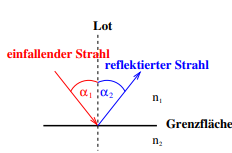
\includegraphics{content/Reflexion.png}
    \caption{Reflexion an einer Grenzfläche\cite{V400}}
    \label{fig:Ref}
\end{figure}
\subsection{Brechung}
Das Phänomen der Brechung tritt auf, wenn Licht in ein anderes Medium mit anderen elektromagnetischen Eigenschaften
eintritt. Die Ausbreitungsgeschwindigkeiten $v$ von Licht unterscheiden sich wegen diesen Unterschieden, bei verschiedenen Materialien.
Beim Übergang zwischen zwei Medien ändert sich daher die Richtung des Lichtstrahls, wie in Abbildung \ref{fig:Bre} dargestellt.
Die Brechung wird durch das Snellius Brechungsgesetz
\begin{equation}
    n_1\cdot \sin{\alpha_1 }=n_2\cdot \sin{\beta }
    \Leftrightarrow \frac{n_1}{n_2}=\frac{v_2}{v_1}=\frac{\sin{\beta}}{\sin{\alpha}}
    \label{eq:Brechung}
\end{equation}
beschrieben, wobei $\alpha$ der Winkel des einfallenden Strahls und 
$\beta$ der Winkel des gebrochenen Strahls zur Flächennormale ist. $n$ ist eine einheitenlose Zahl,
die Brechungsindex genannt wird und das Verhältnis eines Materials zum Vakuum beziehungsweise zu Luft beschreibt.
Der Brechungsindex in Luft entspricht mit $n=1.000292$ fast dem Brechungsindex von 1, also dem Vakuum \cite{V400}.
Das Material mit dem größeren Brechungsindex wird optisch dichter genannt. Beim Übergang in ein optisch dichteres
Material wird ein Lichtstrahl zur Flächennormale hin gebrochen.
\begin{figure}
    \centering
    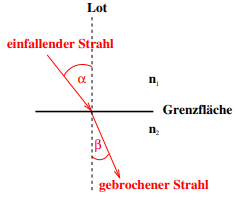
\includegraphics{content/Brechung.png}
    \caption{Brechung beim Übergang in ein optisch dichteres Medium\cite{V400}}
    \label{fig:Bre}
\end{figure}
In Tabelle \ref{tab:BreInd} sind die Brechungsindizes einiger Licht durchlässiger Materialien
aufgelistet.
\begin{table}[H]
    \centering
    \caption{Brechungsindizes verschiedener Stoffe\cite{PhysikTabellen}}
    \label{tab:BreInd}
    \begin{tabular}{c S[table-format=1.6]}
        \toprule
        {Material}&{Brechungsindex $n$}\\
        \midrule
        Luft&1.000292\\
        Wasser&1.333\\
        Kronglas&1.52\\
        Plexiglas&1.49\\
        Diamant&2.42\\
        \bottomrule
    \end{tabular}
\end{table}
\noindent Nun wird ein Objekt mit planparallelen Grenzflächen, das gegenüber Luft optisch dicht ist, betrachtet.
Fällt auf eine solche Platte ein Lichtstrahl, wie in Abbildung \ref{fig:StrV} dargestellt, wird
der Lichtstrahl an beiden Grenzflächen im gleichen Verhältnis einmal hin und einmal weg von der 
Flächennormale gebrochen. Dies resultiert darin, dass der Lichtstrahl im gleichen Winkel die Platte 
verlässt wie er eingetreten ist. Der einzige Unterschied, der durch das hineinbringen der Platte entsteht
ist ein Strahlenversatz $s$, der durch die Formel
\begin{equation}
    s=d\frac{\sin{\alpha-\beta}}{\cos{\beta}}
    \label{eq:Strahlenversatz}
\end{equation}
beschrieben werden kann. Dabei beschreibt $\alpha$ den Einfallswinkel, $\beta$ den Brechungswinkel und $d$
die Dicke der durchlaufenden Platte.
\begin{figure}
    \centering
    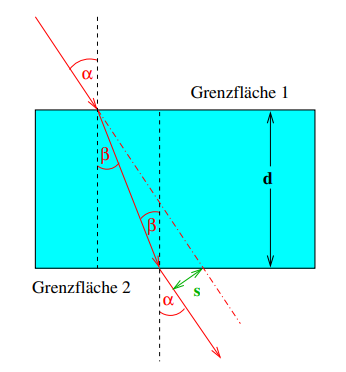
\includegraphics{content/Strahlenversatz.png}
    \caption{Strahlenversatz beim Durchlaufen einer planparallelen Platte\cite{V400}}
    \label{fig:StrV}
\end{figure}
\subsection{Prisma}
Ein Prisma ist ein Objekt mit einem größeren Brechungsindex als Licht, bei dem die Grenzflächen
nicht parallel zueinander stehen. Diese Eigenschaft macht ein Prisma besonders geeignet um die Dispersion von Licht bei
Grenzübergängen zu zeigen. Die Lichtstrahlen unterschiedlicher Wellenlängen werden, auf Grund der verschieden Ausbreitungsgeschwindigkeiten
von Licht im neuen Medium, unterschiedlich stark gebrochen. Dadurch, dass die Grenzflächen nicht parallel sind, wird die Aufspaltung in verschiedene Brechungswinkel
beim Austritt nicht aufgehoben, sondern verstärkt. In Abbildung \ref{fig:Prisma} ist der Strahlengangs eines 
monochromatischen Lichtstrahls dargestellt. Der zugehörige Ablenkwinkel $\delta$ kann
durch die Gleichung
\begin{equation}
    \delta=(\alpha_1+\alpha_2)-(\beta_1+\beta_2)
    \label{eq:Prisma}
\end{equation}
beschrieben werden. $\beta_1$ und $\beta_2$ können über das Brechungsgesetz nach Gleichung \eqref{eq:Brechung} aus $\alpha_1$
und $\alpha_2$, sowie über die Beziehung $\beta_1+\beta_2=\gamma$, bestimmt werden.
\begin{figure}
    \centering
    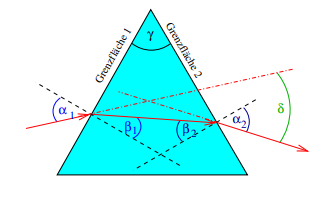
\includegraphics{content/Prisma.png}
    \caption{Darstellung eines Strahlengangs durch ein Prisma\cite{V400}}
    \label{fig:Prisma}
\end{figure}
\subsection{Wellenoptik und Beugung am Gitter}
Gitter sind Objekte, bei denen die undurchlässigen Bereiche in Größenordnungen der Wellenlänge vorliegen.
Bei Licht sollten die Abstände der Spalten im $\unit{\micro\meter}$ Bereich liegen. Dann wirkt jeder Spalt wie eine
Punktquelle für eine Lichtwelle, die alle zueinander kohärent sind, da sie aus der gleichen Ursprungswelle entstanden sind.
Dadurch ergibt sich ein Interferenzmuster. Die konstruktiv interferierenden Stellen, also die Stellen wo sich das Licht aus dem Gitter positiv verstärken,
lassen sich unter einem Winke $\phi$ zum "0-ten Maximum", der Teil des Lichts der mittig senkrecht zum Gitter interferiert, beobachten. Dabei sind Maxima bei verschiedenen Winkeln
beobachtbar. Jedem Maximum wird dabei eine Beugungsordnung $k$ zugeschrieben. Mit größer werdendem Winkel der
Maxima steigt die Beugungsordnung an. Aus den gemessenem Winkel der einzelnen Maxima mit Ordnung $k$ und der Kenntnis des Gitterabstands $d$
lässt sich die Wellenlänge des einfallenden Lichts durch
\begin{equation}
    \lambda=d\frac{\sin{\phi}}{k}
    \label{eq:Beugung}
\end{equation}
bestimmen.
\cite{V400}
